\chapter{Evaluation}

    \section{Datasets}
        In total we used 3 different Datasets (Section \refeq{section:datasets}), which are common used benchmark datasets for evaluating graph neural networks \cite{acharya2019feature, gao2019graphnas, gcn}.
        All of them are citation datasets with nodes being publications and edges representing citations among these publications.        
        Furthermore do all datasets contain nodes' attributes and labels.

        The method to sample the attack dataset $D_A$, described in Section \refeq{subsection:dataset-samples}, follows the common practice in the literature of link prediction \cite{BHPZ17, grover2016node2vec}.

    \section{Metric}
        We use F1-Score as our main evaluation metric.
        It is a common used metric in binary classification \cite{lipton2014thresholding, santus2016features, woodbridge2016predicting}, since it is the harmonic mean of precision and recall.-
        The highest value, that is possible, is 1.0, indicating perfect precision and recall.
        If either the precision or the recall is zero, the F1-Score is 0.0.
        Leading to f1-Score values between 0 and 1.

        \subsection*{Precision}
            A high precision represents a high probability that the prediction of a model is correct.
            Let $M$ be a machine learning model that was trained to predict whether an email is spam or not.
            High precision means, that when the model labels an email as malicious, it is correct most of the time and vice versa.

        \subsection*{Recall}
            A high recall represents a high percentage of correctly classified inputs.
            In the example just given, that means, that $M$ is able to identify a high amount of spam-mails as malicious.


    \section{Attack Performance}
        The results presented below are the average results of 10 runs.
        Meaning, that all attacks have been performed multiple times to get a better relation.
        Note, that the performance varies based on the random choice of the nodes that are included in the partial graph $G_s$.
        Each attack is performed on all target models, which have been trained on different datasets.
        As our baseline we consider that the partial graph $G_s$ doesn't contain any links.
        We then add 20\% of the edges per attack, ending up with 80\% known edges.

        \subsection*{Attack 1}
            Like described in Section \refeq{section:attack1} this attack performs link stealing attacks on the same dataset distribution using the concatenation of the posterior outputs of two nodes to infer whether they have been connected or not. 
            Figure \refeq{figure:eval-att1-citeseer} presents the results for our link stealing attacks on the target models, that have been trained on the CiteSeer dataset.
            The charts for Cora and Pubmed can be found here. \TODO{update}

            \begin{figure}[h]
                \begin{center}
                    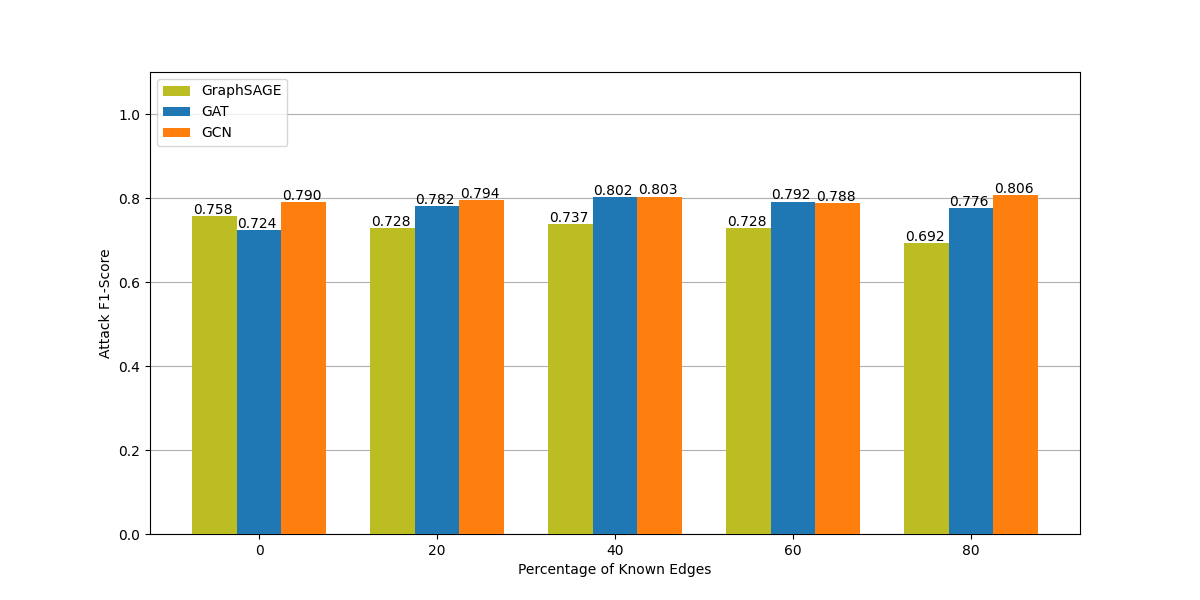
\includegraphics[width=\textwidth]{attack-1-citeseer}
                    \caption{Attack 1 - $D_{f_t} = CiteSeer$}
                    \label{figure:eval-att1-citeseer}
                \end{center}
            \end{figure}

            Note that our baseline already achieves an average F1-Score of $0.7278$ depending on graph neural network type and target dataset $D_{f_t}$.
            The baseline performed best ($0.7605$ F1-Score) on the graphsage graph neural network, when it was trained on the  CiteSeer dataset and it performed worst ($0.6490$ F1-Score) on the graph attention network when it was trained on the Cora dataset.
            Intuitively, with rising amount of known edges, we would expect a higher performance of our attacks.
            However, in most cases, the performance grows until 40\% or 60\% of known edges and drops afterwards.
            More precisely, in almost every case, the attack performance is better with only 60\% of known edges than with 80\%.
            \notsure{The reason we observe this, is the following. Since we use the deleted edges as positive samples for our training data, the more edges are known, the less data will be provided for training the adversary. Leading to more training data in our baseline than in our 80\%-known-edges attack.}
            With respect to all performed attacks, the average F1-Score is $0.7404$, with the lowest being $0.4130$ (GCN trained on Pubmed with 80\% known edges) and the highest being $0.810$ (GraphSAGE trained on CiteSeer with 60\% known edges).

        \subsection*{Attack 2}
            Like described in Section \refeq{section:attack2} this attack performs link stealing attacks on the same dataset distribution using the calculated distance vector of the posterior outputs of two nodes to infer whether they have been connected or not. 
            The following chart presents the results for our link stealing attacks on a target model, that was trained on the CiteSeer dataset.
            The charts for Cora and Pubmed can be found here. \TODO{update}

            \begin{figure}[h]
                \begin{center}
                    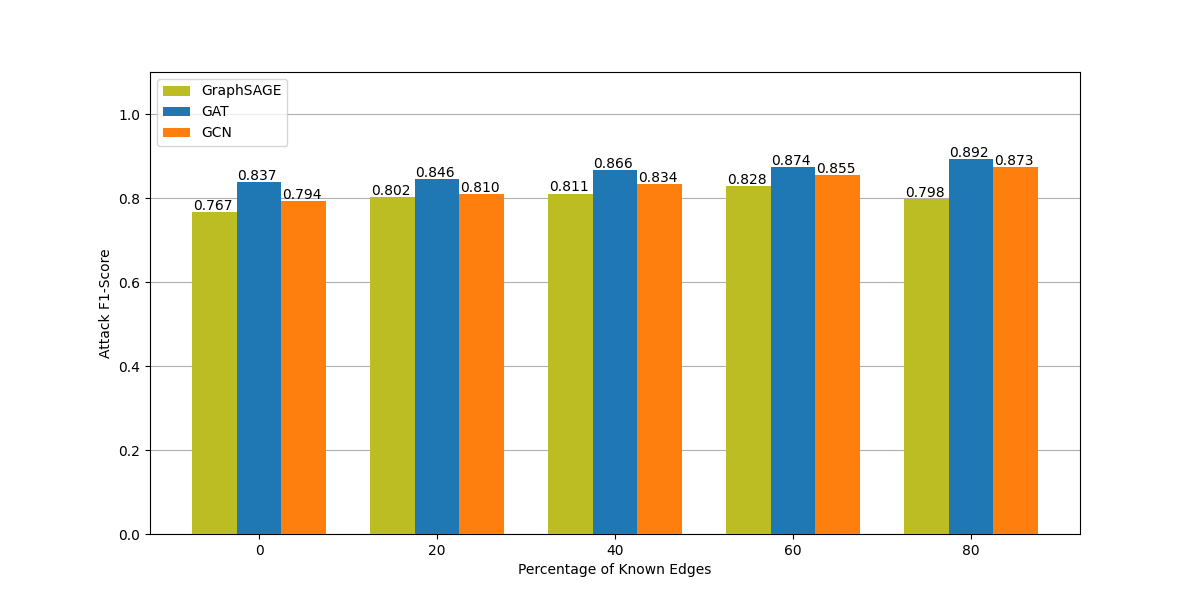
\includegraphics[width=\textwidth]{attack-2-citeseer}
                    \caption{Attack 2 - $D_{f_t} = CiteSeer$}
                    \label{figure:eval-att2-citeseer}
                \end{center}
            \end{figure}

            The first noticeable fact is, that using the distance vector instead of the concatenation of the posteriors is much more effective.
            This time the average F1-Score of our baseline is $0.7715$, again depending on graph neural network type and target dataset $D_{f_t}$.
            The baseline performed best ($0.8355$ F1-Score) on the graphsage graph neural network, when it was trained on the  CiteSeer dataset and it performed worst ($0.6996$ F1-Score) on the graph convolutional network when it was trained on the Cora dataset.
            This time, the results support our forecast.
            With rising amount of known edges, the attack performance grows, leading to an improvement up to 0.06 F1-Score.
            With respect to all performed attacks, the average F1-Score is $0.7969$, with the lowest being $0.6996$ (GCN trained on Cora with 0\% known edges) and the highest being $0.8909$ (GAT trained on CiteSeer with 80\% known edges).

        \subsection*{Attack 3}
            Like described in Section \refeq{section:attack3} this attack performs link stealing attacks on a different dataset distribution using the calculated distance vector of the posterior outputs of two nodes to infer whether they have been connected or not. 
            The following charts present the results for our link stealing attacks on a target model, that was trained on the CiteSeer dataset while the adversary was trained on another distribution dataset.
            The charts for Cora and Pubmed can be found here. \TODO{update}

            \begin{figure}[h]
                \begin{center}
                    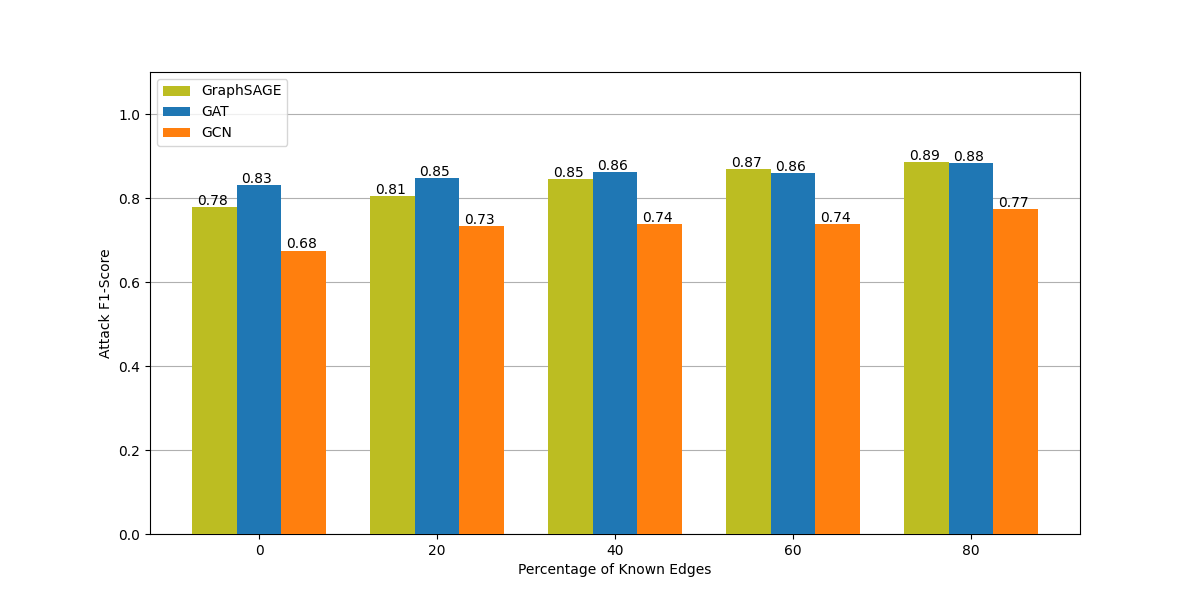
\includegraphics[width=\textwidth]{attack-3-cora-citeseer}
                    \caption{Attack 3 - $D_{f_t} = CiteSeer$ and $D_A = Cora$}
                    \label{figure:eval-att3-citeseer-ora}
                \end{center}
            \end{figure}

            \begin{figure}[h]
                \begin{center}
                    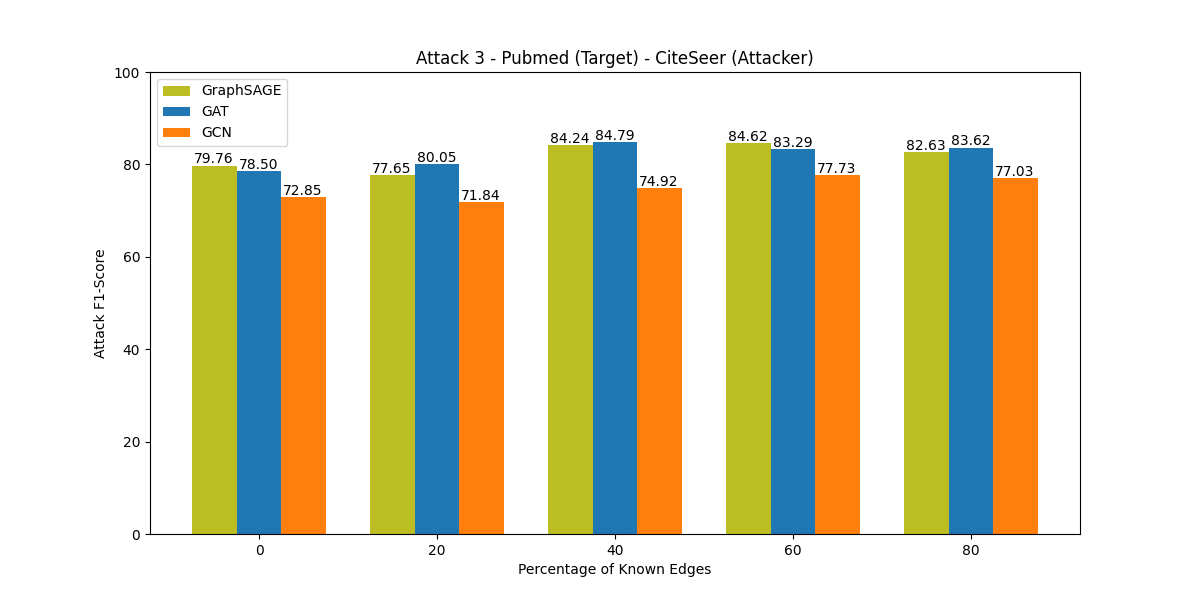
\includegraphics[width=\textwidth]{attack-3-pubmed-citeseer}
                    \caption{Attack 3 - $D_{f_t} = CiteSeer$ and $D_A = Pubmed$}
                    \label{figure:eval-att3-pubmed-cora}
                \end{center}
            \end{figure}
    
    \section{Possible Defense}
        One possible defense, which already has been presented by He et al. \cite{DBLP:journals/corr/abs-2005-02131}, is to minimize the posterior output vector of $f$. 
        Meaning that instead of providing the complete posterior output of $f$'s prediction, $f$ could only present the top $k$ posteriors.
        In that way the adversary must attack the model based on less information which makes the attack less effective.
        
        However, if we assume, that $f$ always provides the complete output posterior, \TODO{finish}

    \section{Summary of Results}
